% Created 2020-10-13 Tue 23:31
% Intended LaTeX compiler: pdflatex
\documentclass[presentation]{beamer}
\usepackage[utf8]{inputenc}
\usepackage[T1]{fontenc}
\usepackage{graphicx}
\usepackage{grffile}
\usepackage{longtable}
\usepackage{wrapfig}
\usepackage{rotating}
\usepackage[normalem]{ulem}
\usepackage{amsmath}
\usepackage{textcomp}
\usepackage{amssymb}
\usepackage{capt-of}
\usepackage{hyperref}
\usepackage[russian]{babel}
\usepackage[T2A]{fontenc}
\usepackage[utf8]{inputenc}
\usepackage{minted}
\usepackage{wrapfig}
\usetheme{Montpellier}
\usecolortheme{rose}
\useinnertheme{rounded}
\author{Макаров Сергей}
\date{\today}
\title{Оптимизация промежуточного представления для абстрактной интерпретации}
\hypersetup{
 pdfauthor={Макаров Сергей},
 pdftitle={Оптимизация промежуточного представления для абстрактной интерпретации},
 pdfkeywords={},
 pdfsubject={},
 pdfcreator={Emacs 27.1 (Org mode 9.3)}, 
 pdflang={Russian}}
\begin{document}

\maketitle

\section{Введение}
\label{sec:orgde2a474}
\begin{frame}[label={sec:org71fac9c}]{Мотивация}
\begin{itemize}
\item В современных решениях для анализа бинарного кода одни и те же задачи, в частности, декодирование команд и трансляция их в промежуточное представление, решаются каждый раз заново, для каждой частной задачи.
\item В рамках проекта Glassfrog предлагается унифицированный подход для решения задач декодирования процессорных команд, трансляции их в промежуточное представление и анализа полученного представления.
\item Для описания форматов файлов, формата и семантики машинных команд предлагается использование внутреннего языка спецификаций с расчётом на то, что поддерживать такие спецификации проще, чем код.
\item В качестве решения для задач анализа кода предлагается подход, основанный на теории абстрактной интерпретации.
\end{itemize}
\end{frame}
\begin{frame}[label={sec:org257d466}]{Glassfrog}
\begin{center}
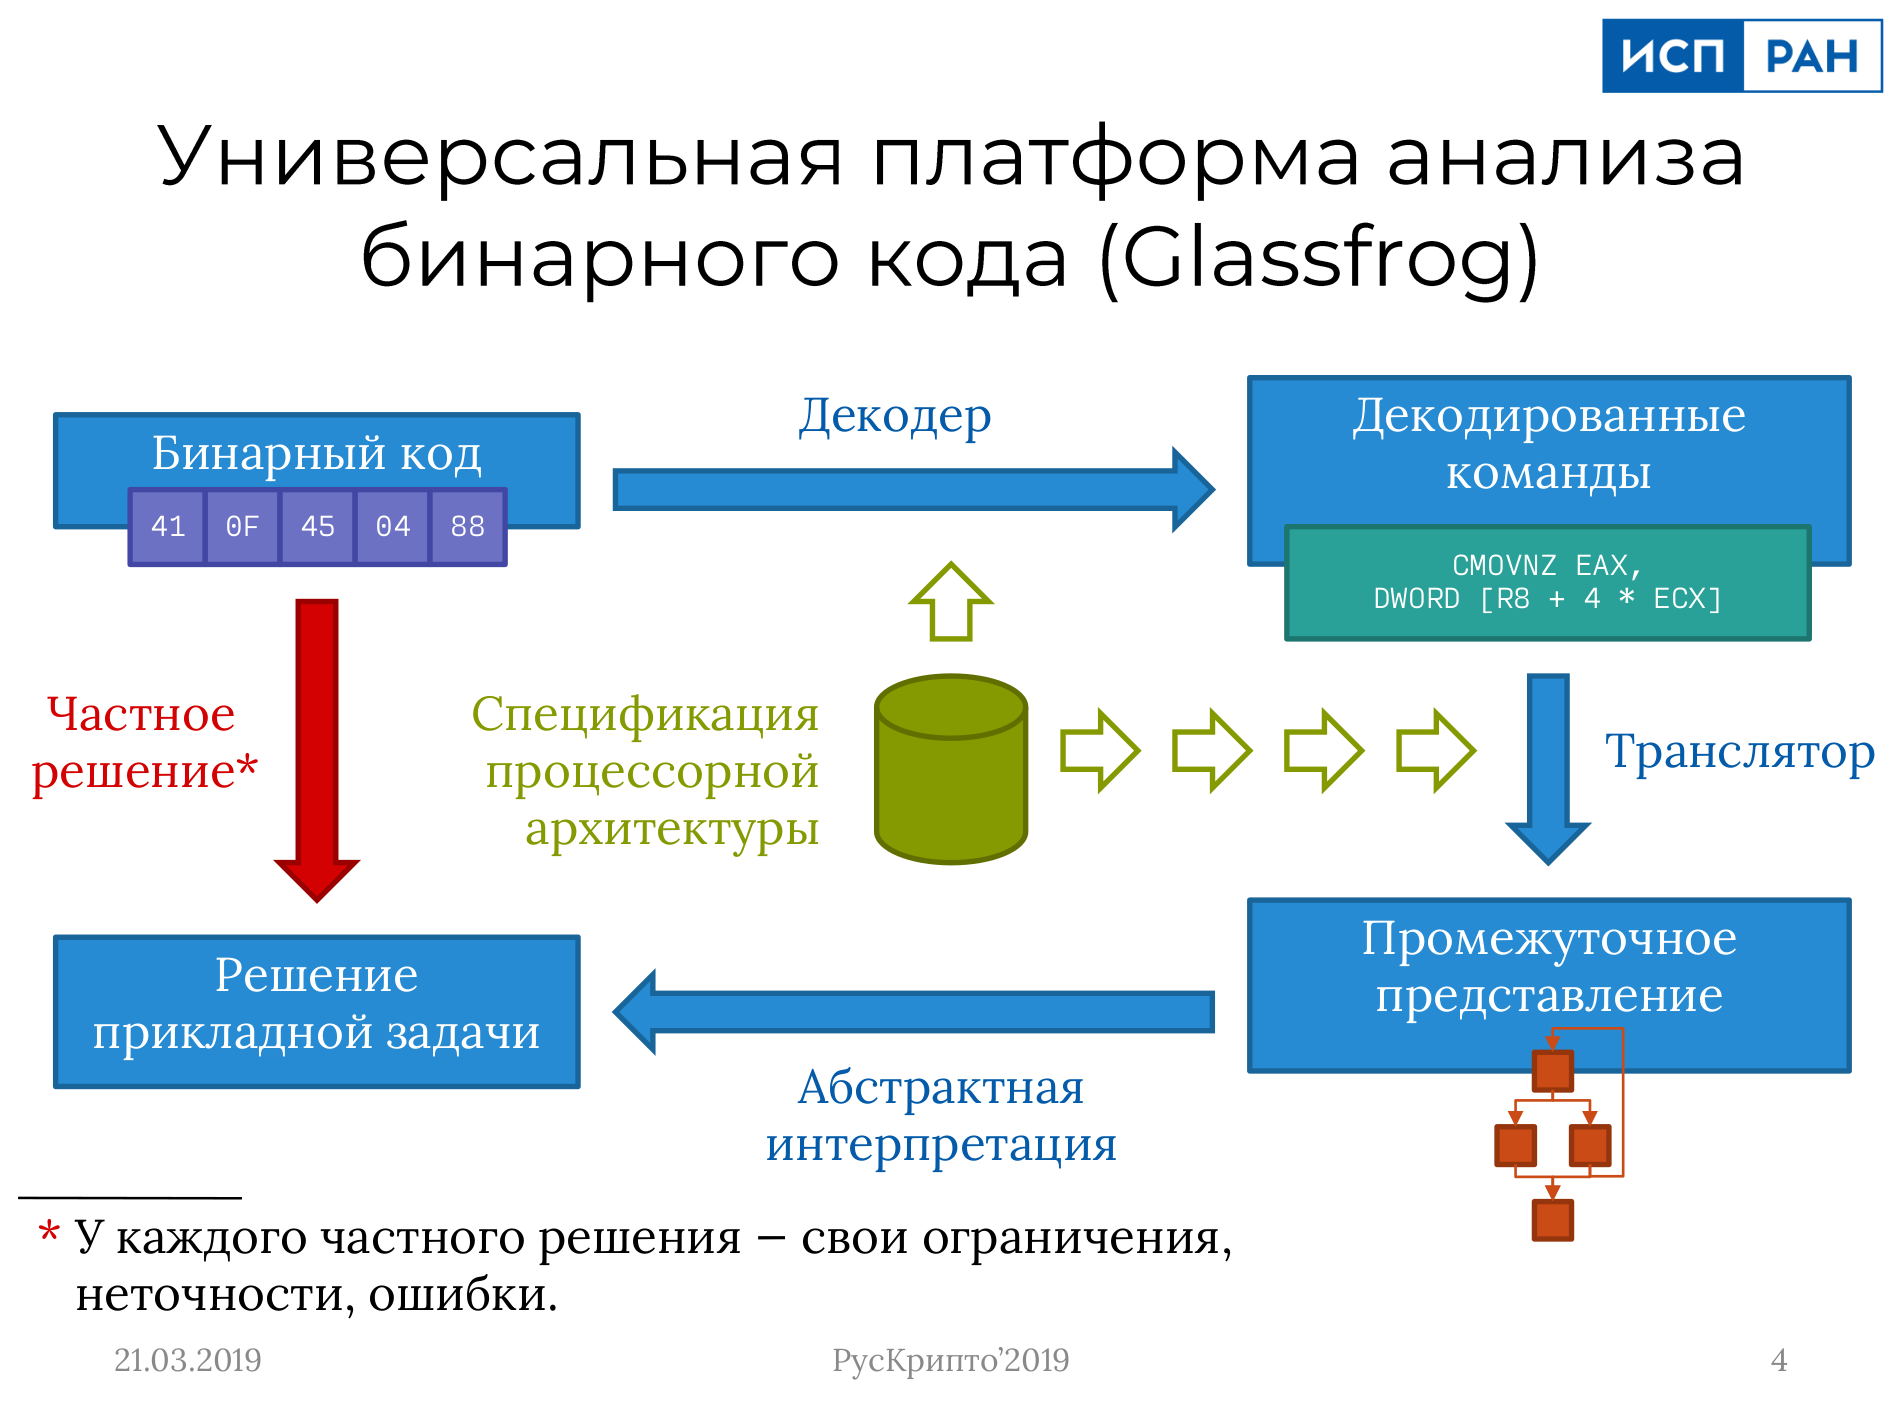
\includegraphics[width=.9\linewidth]{./glassfrog.png}
\end{center}
\end{frame}
\begin{frame}[label={sec:orgf38626f}]{Постановка задачи оптимизации}
Поскольку сложность абстрактной интерпретации напрямую зависит от размера кода, имеет смысл перед абстрактной интерпретацией провести некоторые оптимизации, чтобы уменьшить размер промежуточного представления. Есть две возможности для оптимизации сгенерированного кода:
\begin{enumerate}
\item Оптимизация при компиляции спецификаций.
\item Оптимизация при построении промежуточного представления.
\end{enumerate}
\end{frame}
\begin{frame}[label={sec:org85279e6}]{Структура Pivot2 IR}
\begin{itemize}
\item Модули
\item Адресные пространства
\item Константы
\item Базовые блоки
\item Фрагменты
\end{itemize}
\end{frame}
\begin{frame}[label={sec:org81dfffe},fragile]{Фрагменты}
 \begin{itemize}
\item Фрагмент представляет собой гамак из базовых блоков.
\item Фрагмент представляется в SSA форме. Передача переменных по рёбрам CFG осуществляется с помощью входных и выходных переменных базовых блоков.
\item Переменные базовых блоков имеют областью видимости весь фрагмент.
\item Базовые блоки представляют собой последовательность операторов. Всего есть 7 операторов: \texttt{APPLY}, \texttt{CALL}, \texttt{INIT}, \texttt{LOAD}, \texttt{MIX}, \texttt{SLICE} и \texttt{STORE}.
\end{itemize}
\end{frame}
\section{Оптимизация спецификаций}
\label{sec:org22427e6}
\begin{frame}[label={sec:org32e937e}]{Общая структура оптимизаций}
\begin{center}
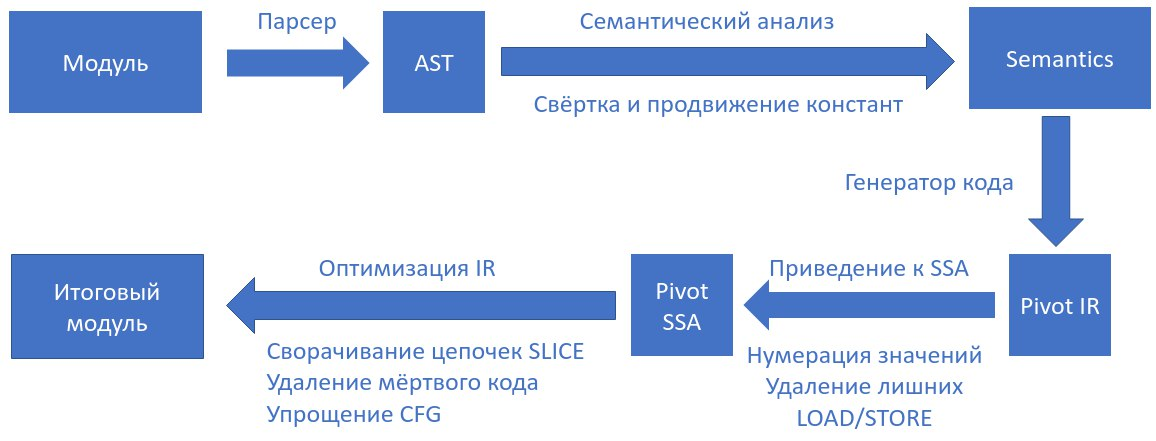
\includegraphics[width=.9\linewidth]{./compiler.jpg}
\end{center}
\end{frame}
\begin{frame}[label={sec:orgc590b15},fragile]{Свёртка и продвижение констант}
 \begin{figure}
\begin{minipage}[t]{0.4\textwidth}
\begin{minted}[]{rust}
let y = 2;
let x = if y {
    'add(1, 2)
} else {
    'sub(2, 1)
};
\end{minted}
\end{minipage}%
\begin{minipage}[t]{0.2\textwidth}
$$\Longrightarrow$$
\end{minipage}%
\begin{minipage}[t]{0.4\textwidth}
\begin{minted}[]{rust}
let y = 2;
let x = 3;   
\end{minted}
\end{minipage}%
\end{figure}
\end{frame}
\begin{frame}[label={sec:org39c47eb},fragile]{Построение SSA}
 \begin{figure}
\begin{minipage}[t]{0.4\textwidth}
\begin{minted}[]{rust}
fn fact(n: v32) -> v32 {
    let v = 1;
    while 'ne(n, 0) {
        v = 'mul(v, n);
        n = 'sub(n, 1);
    }
    v
}
\end{minted}
\end{minipage}%
\begin{minipage}[t]{0.2\textwidth}
$$\Longrightarrow$$
\end{minipage}%
\begin{minipage}[t]{0.4\textwidth}
\begin{minted}[,fontsize=\footnotesize]{asm}
fn fact(n: v32) -> v32 {
    INIT(v0, 1);
    OUTPUT n;
    OUTPUT v0;
L1: INPUT v1;
    INPUT v2;
    INIT(v3, 0);
    APPLY(v4, ne, v1, v3);
    IF v4 JMP L2;
    APPLY(v5, mul, v2, v1);
    INIT(v6, 1);
    APPLY(v7, sub, v1, v6);
    OUTPUT v7;
    OUTPUT v5;
    JMP L1;
L2: OUTPUT v1    
}
\end{minted}
\end{minipage}%
\end{figure}
\end{frame}
\begin{frame}[label={sec:org931c68d},fragile]{Удаление лишних подвыражений}
 \begin{figure}
\begin{minipage}[t]{0.4\textwidth}
\begin{minted}[,fontsize=\scriptsize]{asm}
space regs(v32);

fn fact(n: v32) -> v32 {
    INIT(v0, 1);
    INIT(v1, 0);
    STORE(regs, v1, v0);
    OUTPUT n;
    OUTPUT v0;
L1: INPUT v2;
    INPUT v3;
    INIT(v4, 0);
    APPLY(v5, ne, v2, v4);
    IF v5 JMP L2;
    APPLY(v6, mul, v3, v2);
    INIT(v7, 1);
    APPLY(v8, sub, v2, v7);
    LOAD(v9, regs, v4);
    OUTPUT v8;
    OUTPUT v6;
    JMP L1;
L2: OUTPUT v2
}
\end{minted}
\end{minipage}%
\begin{minipage}[t]{0.2\textwidth}
$$\Longrightarrow$$
\end{minipage}%
\begin{minipage}[t]{0.4\textwidth}
\begin{minted}[,fontsize=\scriptsize]{asm}
space regs(v32);

fn fact(n: v32) -> v32 {
    INIT(v0, 1);
    INIT(v1, 0);
    STORE(regs, v1, v0);
    OUTPUT n;
    OUTPUT v0;
L1: INPUT v2;
    INPUT v3;
    APPLY(v5, ne, v2, v1);
    IF v5 JMP L2;
    APPLY(v6, mul, v3, v2);
    APPLY(v8, sub, v2, v7);
    LOAD(v9, regs, v4);
    OUTPUT v8;
    OUTPUT v6;
    JMP L1;
L2: OUTPUT v2
}
\end{minted}
\end{minipage}%
\end{figure}
\end{frame}
\begin{frame}[label={sec:org5fcce6c},fragile]{Удаление лишних LOAD/STORE}
 \begin{figure}
\begin{minipage}[t]{0.4\textwidth}
\begin{minted}[,fontsize=\scriptsize]{asm}
space regs(v32);

fn fact(n: v32) -> v32 {
    INIT(v0, 1);
    INIT(v1, 0);
    STORE(regs, v1, v0);
    OUTPUT n;
    OUTPUT v0;
L1: INPUT v2;
    INPUT v3;
    APPLY(v5, ne, v2, v1);
    IF v5 JMP L2;
    APPLY(v6, mul, v3, v2);
    APPLY(v8, sub, v2, v7);
    LOAD(v9, regs, v4);
    OUTPUT v8;
    OUTPUT v6;
    JMP L1;
L2: OUTPUT v2
}
\end{minted}
\end{minipage}%
\begin{minipage}[t]{0.2\textwidth}
$$\Longrightarrow$$
\end{minipage}%
\begin{minipage}[t]{0.4\textwidth}
\begin{minted}[,fontsize=\scriptsize]{asm}
space regs(v32);

fn fact(n: v32) -> v32 {
    INIT(v0, 1);
    INIT(v1, 0);
    STORE(regs, v1, v0);
    OUTPUT n;
    OUTPUT v0;
L1: INPUT v2;
    INPUT v3;
    APPLY(v5, ne, v2, v1);
    IF v5 JMP L2;
    APPLY(v6, mul, v3, v2);
    APPLY(v8, sub, v2, v7);
    OUTPUT v8;
    OUTPUT v6;
    JMP L1;
L2: OUTPUT v2
}
\end{minted}
\end{minipage}%
\end{figure}
\end{frame}
\begin{frame}[label={sec:orgfd5884c}]{Расширенные базовые блоки}
\begin{wrapfigure}{l}{0.3\textwidth}
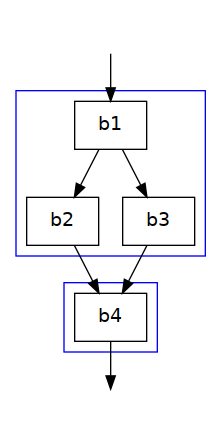
\includegraphics[height=150px]{cfg-ebb.png}
\end{wrapfigure}
Любое выражение, вычисляемое в блоке b1, может быть использовано в блоках b2 и b3. 
\alert{Можно ли использовать этот факт, чтобы улучшить описанные оптимизации?}
\end{frame}
\begin{frame}[label={sec:orgb1116fc},fragile]{Обход расширенных базовых блоков}
 \begin{minted}[]{text}
entries = CFG.entry;

while entries is not empty {
    current_entry = entries.pop();
    DFS(current_entry) // Stop at join nodes
                       // add join nodes to entries;
}
\end{minted}

Используя этот алгоритм, мы получим обход расширенных базовых блоков в порядке обхода в глубину, вершины каждого расширенного блока будут также обходиться в глубину.

\alert{Не нарушает ли такой обход корректности алгоритма построения SSA?}
\end{frame}
\begin{frame}[label={sec:org9481d54},fragile]{Обобщение методов оптимизации}
 \begin{minted}[]{text}
for each EBB in CFG {
    value numbers = {};
    memory vars = {};
    for each block in EBB {
        on enter {
            add new layer to value numbers;
            add new layer to memory vars;
            translate block to SSA;
        }
        on leave {
            remove last layer from value numbers;
            remove last layer from memory vars;
        }
    }
}   
\end{minted}
\end{frame}
\begin{frame}[label={sec:org329ef1e},fragile]{Сворачивание цепочек операторов SLICE}
 \begin{figure}
\begin{minipage}[t]{0.4\textwidth}
\begin{minted}[]{rust}
if a {
    s[0:17][0:3]
} else {
    s[17:34][0:3]
}
\end{minted}
\end{minipage}%
\begin{minipage}[t]{0.2\textwidth}
$$\Longrightarrow$$
\end{minipage}%
\begin{minipage}[t]{0.4\textwidth}
\begin{minted}[]{rust}
if a {
    s[0:3]
} else {
    s[17:20]
}
\end{minted}
\end{minipage}
\end{figure}
\end{frame}
\begin{frame}[label={sec:orga9540cc},fragile]{SliceForest}
 \begin{figure}
\begin{minipage}[t]{0.5\textwidth}
\begin{minted}[]{asm}
    INPUT a;
    INPUT s;
    IF a JMP L1;
    SLICE(v0, s, 17, 34);
    SLICE(v1, v0, 0, 3);
    OUTPUT v1;
    JMP L2;
L1: SLICE(v2, s, 0, 17);
    SLICE(v3, v2, 0, 3);
    OUTPUT v3;
L2: INPUT v4
    OUTPUT v4
\end{minted}
\end{minipage}
\begin{minipage}[t]{0.2\textwidth}
\begin{center}
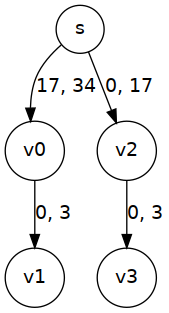
\includegraphics[height=150px]{slice-forest.png}
\end{center}

\end{minipage}
\end{figure}
\end{frame}
\begin{frame}[label={sec:org6eb6021}]{Сжатие ветвей}
\begin{figure}
\begin{minipage}[t]{0.4\textwidth}
\begin{center}
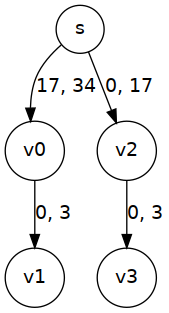
\includegraphics[height=150px]{slice-forest.png}
\end{center}
\end{minipage}
\begin{minipage}[t]{0.4\textwidth}
\begin{center}
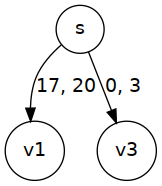
\includegraphics[height=100px]{slice-forest-compressed.png}
\end{center}

\end{minipage}
\end{figure}
\end{frame}
\begin{frame}[label={sec:org52d79bb}]{Удаление мёртвого кода и упрощение CFG}
Удаление мёртвого кода производится с помощью классического Mark\&Sweep алгоритма. На первой фазе помечаются все важные операторы и переходы, на второй фазе непомеченные операторы удаляются.

Упрощение CFG достигается посредством систематического применения четырёх трансформаций:
\begin{enumerate}
\item Замена ветвления, оба ребра которого переходят в один блок, на безусловный переход.
\item Удаление пустого блока.
\item Слияние двух подряд идущих блоков.
\item Перенос ветвления из пустого блока к предку.
\end{enumerate}
\end{frame}
\section{Оптимизация анализируемого кода}
\label{sec:orgdcdf513}
\begin{frame}[label={sec:org77113a4}]{Абстрактная интерпретация}
В терминах Glassfrog интерпретация это абстрактное состояние и набор передаточных функций, определяющих, как изменяется состояние при выполнении каждого оператора и при переходе по ребру CFG. Для задач анализа потока данных интерпретация должна быть монотонна, т. е. множество её состояний должно образовывать решётку и все передаточные функции должны быть монотонны относительно порядка, введённого этой решёткой. Вычисление результата абстрактной интерпретации по фрагменту происходит с помощью исполнителя.
\end{frame}
\begin{frame}[label={sec:org08d9138},fragile]{Глобальное удаление избыточного кода}
 С помощью абстрактной интерпретации находятся множества доступных выражений и содержимое памяти в начале каждого блока. Следующий проход заменяет лишние вычисления, чтения и записи на операторы \texttt{MIX}, используя эту информацию. Наконец, последним проходом удаляются операторы \texttt{MIX}.
\begin{enumerate}
\item Передаточная функция для операторов \texttt{APPLY}, \texttt{INIT} и \texttt{SLICE} добавляет соответствующее выражение как доступное.
\item Передаточная функция для оператора \texttt{STORE} обновляет содержимое соответствующей ячейки памяти.
\item Передаточная функция для оператора \texttt{CALL} сбрасывает наборы доступных выражений и содержимое памяти.
\end{enumerate}
\end{frame}
\section{Заключение}
\label{sec:org8d9902e}
\begin{frame}[label={sec:org505eaac}]{Заключение}
\begin{itemize}
\item Были реализованы два пакета набора оптимизаций: для оптимизации спецификаций процессорных архитектур и для оптимизации анализируемого представления.
\item Замеров того, насколько реализованные оптимизации повышают скорость анализа, не производилось, поскольку соответствующая инфраструктура ещё не до конца реализована, и не набрана достаточная база примеров.
\item В дальнейшем планируется реализовать на основе инфраструктуры поиск утечек и пополнить базу примеров и спецификаций.
\end{itemize}
\end{frame}
\begin{frame}[label={sec:orgf210d03}]{Источники}
\begin{itemize}
\item \url{https://ispranproceedings.elpub.ru/jour/article/view/1120} \\
\item K. Cooper, L. Torczon, Engineering a Compiler 2nd Edition \\
\item \url{https://compilers.cs.uni-saarland.de/papers/bbhlmz13cc.pdf} \\
\item \url{http://www.di.ens.fr/\~cousot/COUSOTpapers/POPL77.shtml} \\
\item \url{https://ispranproceedings.elpub.ru/jour/article/view/1257}
\end{itemize}
\end{frame}
\end{document}
